\chapter{Caption Generation Pipeline: \\Model and Evaluation}
\chaptermark{Baseline Model \& Evaluation Metrics}
\label{chapter:baseline}
%%===========================================================================%%
In this chapter, we will examine in detail all the constituent parts
of training an image captioning system.
%%
First we will look at a baseline captioning model adapted from
\cite{Vinyals_2015_CVPR}. 
%%
Although the original model was proposed for generating captions for still
images, the same architecture can be used for video captioning, by
swapping out the image feature extraction module with video feature extraction
module.
%%
Thus the discussion presented here is kept generic, and specific details of
features used for image or video captioning is discussed in
Chapter~\ref{chapter:VisFeatChapter}.
%%

We will then discuss some popular datasets which are used to train the
captioning models and discuss the salient aspects of each dataset.
%%
We will also discuss the metrics used to evaluate captions generated by the
models. 

The model presented in this chapter acts as the baseline against which we
compare the performance of the architectures we propose in the rest of the
thesis.

\section{Baseline Architecture} 

Our caption generation model consists of two stages: the visual
feature extraction stage followed by a language model
%%
In the first stage, we use various techniques to extract descriptors of
the visual contents of input image or video.
%%
These descriptors are then represented as one or more vectors of fixed
dimension.
%%
The language model then uses these feature vectors and generates a
suitable caption to describe the image.
%%
This pipeline is illustrated in Figure~\ref{fig_fullModel}. 
%%

In the following subsections we will give an overview of the different image
features and the language model used in the baseline architecture.

\begin{figure}[t]
  \begin{center}
      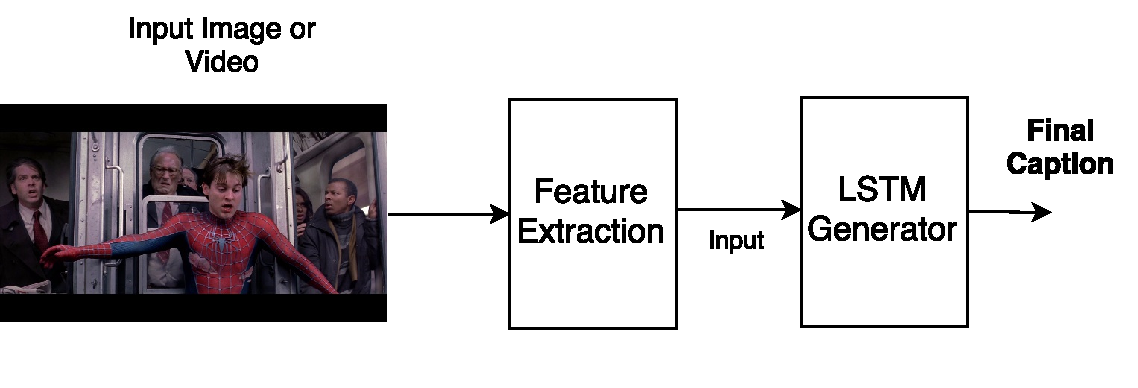
\includegraphics[width=0.8\linewidth]{images/Thesis_generalBaseline.pdf}
  \end{center}
  \vspace*{-8mm}
  \caption{Block diagram showing our image captioning pipeline from an
  input image to the generated caption.}
  \label{fig_fullModel}
\end{figure}

\subsection{Visual Feature Extraction}

\paragraph{Baseline image feature}: As discussed in \ref{chapter2:visFeat},
image features extracted from CNNs pre-trained on ImageNet have become
ubiquitous in most image understanding tasks.
%%
Thus in our baseline captioning model, we use features extracted from
GoogleLeNet~\cite{DBLP:journals/corr/SzegedyLJSRAEVR14} as the image feature
vector. 
%%
More details of the feature extraction process are discussed in
chapter~\ref{chapter:VisFeatChapter}, but it suffices to say here that feature
vectors are formed by the activations of the \emph{5th Inception module} in
GoogeleLeNet.
%%
After concatenating such activations extracted from different
poolings of image crops, we obtain a feature vector of 4096 dimensions.

\paragraph{Baseline video feature}: As a very simple baseline feature vector for
videos, we use the same GoogleLeNet features as above, but extracted only on the
key-frame of the video.
%%
Key-frame is taken as the frame at the center of video's timespan.
%%
The main idea behind this simple feature vector is to enable video captioning
baseline model to use the same pipeline as the image and obtain a reasonable
baseline against which more sophisticated feature extraction methods can be
compared. 

%%----------------------------------%%
\subsection{Language Model}

The next stage in the pipeline is a conditional language model which
takes as input the image features and generates a caption. 
%%
Long-Short Term Memory (LSTM) networks~\cite{Hochreiter1997} have been a popular
choice in the literature to model the probability of a sentence $S$ given an
image $I$ as $P(S|I)$.
%%

\subsubsection{LSTM Cell}

\begin{figure}[h]
  \begin{center}
    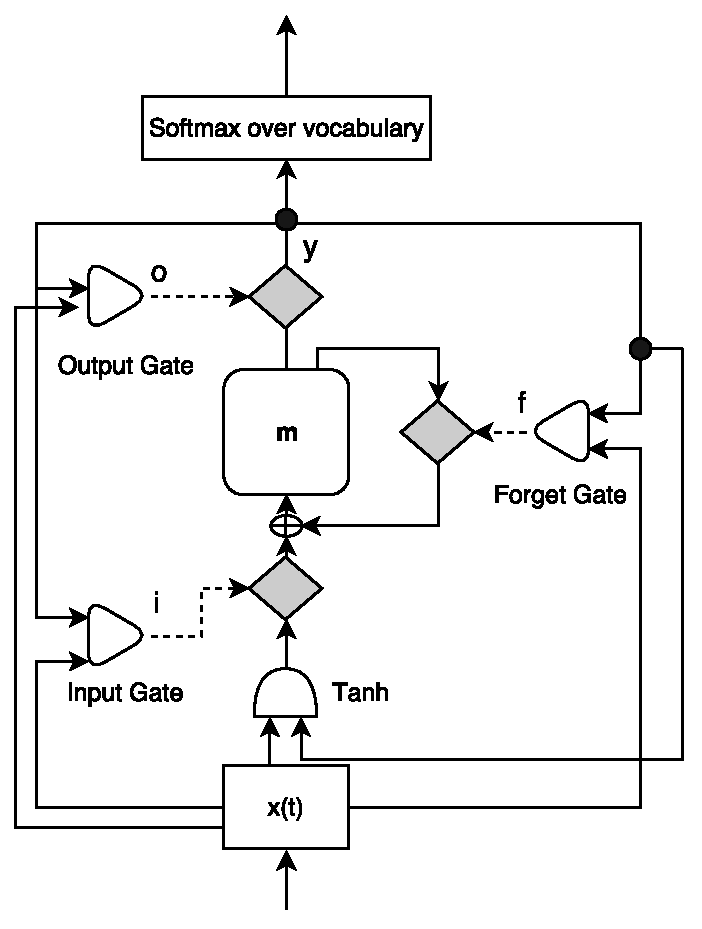
\includegraphics[width=0.5\linewidth]{images/LstmBlockDiag.pdf}
  \end{center}
  \vspace*{-6mm}
  \caption{A single LSTM cell is shown here. Dotted lines
    to the rhombi indicate multiplications as gate controls and the
    solid lines depict the data flow. Triangles are sigmoid
    non-linearities.}
  \label{fig:lstmcell}
\end{figure}

The LSTM model is chosen for this task based on two basic requirements the image
captioning problem imposes. 
%%
Firstly, the language model needs to handle sentences of arbitrary length and
LSTMs are able to do this by design.
%%
Secondly, during the training with gradient descent methods, the error
signal and its gradients need to propagate a long way back in time
without exploding, and again LSTMs satisfy this criteria.

The block diagram of a single LSTM cell is shown in
Figure~\ref{fig:lstmcell}.  
%5
It consists of a memory cell $m$, whose value at any time step $t$ is
influenced by the current vectorial input $x$, the previous output
$y(t-1)$ and the previous cell state $m(t-1)$.
%%
The update to the memory value $m$ is controlled using the input gate
$i$ and the forget gate $f$.
%%
The output is controlled using the output gate $o$. 
%%
The gates are implemented with sigmoidal non-linearities
$\sigma(\cdot)$ to keep them completely differentiable.
%%
The input and forget gates of the LSTM cells have the ability to
preserve the content of the memory cell over long periods, which makes
it easier to learn longer sequences.
%%
This process is formalized in the equations:
%%
\begin{align}
  \label{eqn:lstmstrt}
  i(t) &= \sigma(W_{ix}x(t-1) + W_{iy}y(t-1))\\
  o(t) &= \sigma(W_{ox}x(t-1) + W_{oy}y(t-1))\\
  f(t) &= \sigma(W_{fx}x(t-1) + W_{fy}y(t-1))\\
  \label{eqn:lstmend}
  \begin{split}
    m(t) &= f(t)\cdot m(t-1) \:\, + \\
    &\; \; \; \; \; i(t)\cdot \tanh(W_{mx}x(t)+W_{my}y(t-1))
  \end{split}\\
  y(t) &= o(t) \cdot m(t) \;,
\end{align}
%%
where $W_{\cdot\cdot}$ are the network weights learned during the
training phase.

%% --------------------------------------

\subsubsection{Basic LSTM Language Model}
\label{subsec:basiclstmodel}

Our baseline LSTM language model is based on the network proposed
in~\cite{Vinyals_2015_CVPR}.
%%
The block diagram of this language model is shown in
Figure~\ref{fig:baselinelstmlang}
%%
The model consists of an LSTM network with a softmax layer at its
output. 
%%
The softmax outputs the probability distribution over the model's
vocabulary as:
%%
\begin{align}
p(w_t | w_{t-1},\cdots,w_0, V) = \text{softmax}(W_d y(t)) \;.
\end{align}
\noindent where $W_d$ is the decoder matrix of which maps vector $y(t)$, which
is the same size as number of LSTM units used, to the vocabulary size.
%%

The visual features $V$ are fed into the LSTM through a
embedding matrix $W_{ix}$ at the zeroth time step as the input $x(0)$.
%%
We refer to this feature input as the \emph{init} feature since it
initializes the hidden state of the LSTM.
%%
In the subsequent time steps, a start symbol followed by the word
embeddings for each word in the reference caption (during training) or
the previous generated word (during testing) are fed through the same
input line, as $x(t)$.

During the training phase, at each time step, the LSTM is trained to
assign the highest probability to the next ground truth word given the
current inputs and the hidden state.
%%
This is done by maximizing the log probability assigned to the training 
samples by the model. Equivalently, we can minimize the negative log likelihood 
given as:
%%
\begin{align}
  \label{eqCost}
  L(w_{1\cdots L} | V) = -\sum_{t=1}^n \log(p(w_t|w_{t-1},V)) \; .
\end{align}
%%
\begin{figure}[h]
\begin{center}
   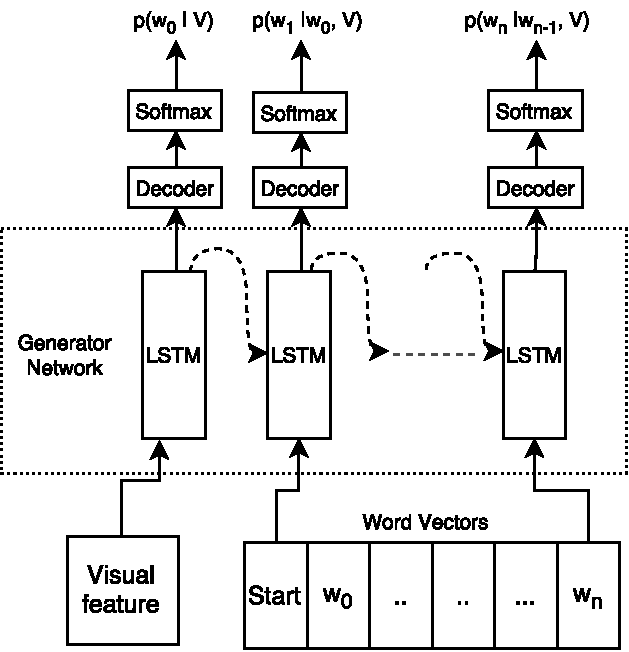
\includegraphics[width=0.5\linewidth]{images/Thesis_lstmLangGen.pdf}
\end{center}
\vspace*{-4mm}
\caption{Baseline LSTM based language model is shown here with
  LSTMs unrolled in time.}
\label{fig:baselinelstmlang}
\end{figure}

\subsection{Training and Regularization}
%%----------------------------------%%
Training the network involves tuning the parameters of the language model
in-order to maximize the log likelihood cost function shown in Eq~\ref{eqCost}.
%%
This optimization is achieved by backpropagating the cost through time and
adjusting the LSTM parameters using gradient descent.
%%
Specifically we use stochastic gradient descent with the
RMSProp~\cite{rmspropTielman} algorithm.
%%
The training samples are used in random mini batches of sentence-image pairs,
and gradient descent is done after accumulating the cost for each mini batch. 

All the LSTM parameters, the word embedding vectors and decoder matrix are
learnt using this method.
%%
But the parameters of feature extraction modules are not trained and are held
fixed in order to prevent overfitting. 
%%
This is necessary as usually the feature extraction modules, e.g. image CNN
network, are powerful models pre-trained on large datasets and can easily
overfit on the relatively small datasets like the ones used in captioning.

We use dropout for regularization in the LSTM language model.
\cite{ZarembaSV14}.
%%
Here dropout is only applied on the input and output of LSTM and not on
the recurrent connections.
%%
We find that dropout, with a drop probability of 0.5, greatly improves model
generalization.
%%
Word embedding vectors and decoder matrix are regularized by adding a penalty to
minimize their l2 norm.

\subsection{Test Mode: Beam Search}
%%
In the caption generation phase for test images,we don't have a reference
caption and need to sample from the distribution $p(S|I)$, to generate the
caption.
%%
Similar to the training phase, the image feature vector is fed into the LSTM
network at time-step 0 followed by the 'START' symbol.
%%
Now, at time-step $t=1$, the word with highest probability at the softmax output
is the word the model thinks is the most likely first word.
%%
Thus we pick this as the generated word and feed the word vector for this word
as the input to the LSTM in the next time step, $t=2$.
%%
This process is repeated until the model produces a period symbol('.').
%%
That marks the end of generation process and we have a candidate sentence.
%%

One problem here is that if we only consider the most likely word at each
time-step we are not guaranteed to get the most likely sentence.
%%
Ideally we need to have an approach like dynamic programming and search the
entire space  of possible sentences.
%%
But this is intractable.
%%
A good approximation is to use beam-search, wherein we maintain top k partial
sentences at each step.
%%
For each of these top-k sentences we consider extensions with top-k words and
re-score the candidates.
%%
Of these $k^2$ possibilities only best k extensions are preserved.
%%
This process is repeated until all the search beams terminate or maximum allowed
sentence length is reached.
%%
At the end of this process we have k generated candidate sentences ranked
according to the log-probability assigned by the model.
%%

\section{Evaluation Metrics}
\label{sec:EvaluationMetrics}
The evaluation of a captioning system is not trivial, due to the
\red{multiple} nature of the problem.
%%
An image can be correctly described with wide variety of captions differing not
only in the syntactic structure of the caption, but also in the semantic content
of it.
%%
We can see an example of this in figure~\ref{fig_capdiversity}, where a sample
image from MS-COCO training set is shown with the corresponding ground truth
captions.
%%
Here we see that each caption focusses on different aspects of the image, from
the \emph{big rock} to \emph{crystal blue water}.
%%
But all the captions are equally valid.
%%

A possible method of evaluation is to compare the machine generated
caption with the target reference captions.
%%
But, we need to note that the reference captions only represent few samples from
the space of all valid captions for input image.
%%
Thus the evaluation metrics we use to measure the correctness of a machine
generated caption should be able to take these issues into account.

\begin{figure}[h]
    \begin{minipage}[c]{0.45\linewidth}
        %\begin{center}
            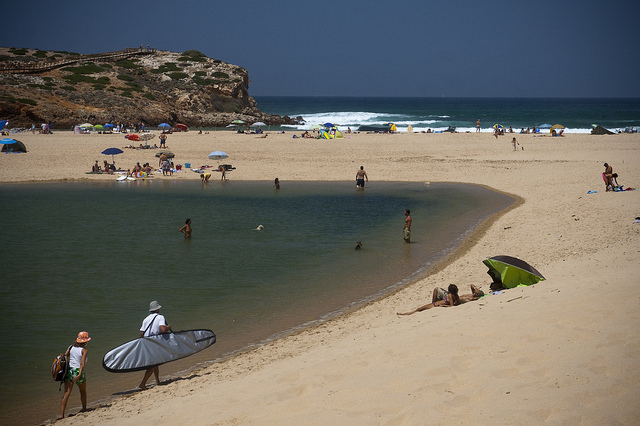
\includegraphics[width=\textwidth]{images/COCO_train2014_000000440903.jpg}
        %\end{center}
    \end{minipage}\hfill
    \begin{minipage}[c]{0.52\linewidth}
            \textbf{C1:} a beach with people relaxing on a \red{sunny day}. \\
            \textbf{C2}: people are relaxing on the beach where there is a \red{big rock}. \\
            \textbf{C3}: a beach with a group of people with surf boards and \red{umberellas}. \\
            \textbf{C4}: a group of people enjoy a beach near a lagoon filled with \red{crystal blue
            water}. \\
            \textbf{C5}: a \red{man walking} on a beach with his surf board in a case. \\
    \end{minipage}
  \vspace*{-3mm}
  \caption{ A sample image from the training set with associated ground truth
  captions. Here we see a clear case where different captions focus on different
  aspects of the image.
  }
  \label{fig_capdiversity}
\end{figure}

One aspect of this problem, the syntactic variations in target sentences, is also
seen in the well--studied field of machine translation.
%%
In this case, a sentence in one language could potentially be translated into
multiple valid sentences in the desired language.
%%
But machine translation differs from image captioning by the fact that, although
these multiple translations can differ syntactically, they tend to have the same
semantic content.

Nevertheless, image captioning literature has borrowed three evaluation metrics
popular in machine translation, namely BLEU\cite{Papineni:BLEU},
ROUGE-L\cite{lin2004rouge} and METEOR\cite{denkowski-lavie:2014:Meteor}. 
%%
Another metric popular in image captioning evaluation is the CIDEr metric which
was proposed recently in \cite{Vedantam_2015_CVPR}, specifically for this task. 
%%
Next we will discuss each of these four metrics briefly to better understand
what exactly they measure.

\subsection{BLEU}
BLEU is a simple metric which scores captions based on the n-gram matches
between the candidate and the reference captions.
%%
First, the total
number of occurences of a word in the candidate sentence, clipped to it's
maximum occurence in a single reference sentence, is accumulated.
%%
Next a modified precision score is computed by dividing this accumulated score
by the total number of words in the candidate.
%%
This process is repeated for different n-grams, yielding modified precision
scores $p_n$. 
%%
Final Bleu score is given by:
\begin{equation}
    BLEU-N = BP\cdot{}exp(\sum_{n=1}^{N}w_{n}log(p_n))        
\end{equation}

\noindent where BP is the brevity penalty applied in-order to penalize 
short candidate sentences.
%%
This additional term is required since, if we only use precision, degenerate
candidates like the one containing just single words will always score better.

In image captioning evaluation, BLEU-1 to BLEU-4 have been used. 
%%
\subsection{ROUGE-L}
ROUGE metrics were proposed for evaluating text summaries.
%%
The version used in image captioning evaluation is ROUGE-L, a metric based on
recall and precision scores of longest common subsequences~(LCS) between the reference
and candidate sentences.
%%
\begin{align}
        R_{lcs} &= \frac{LCS(C,Ref)}{Refernce\ length}\\[0.75ex]
        P_{lcs} &= \frac{LCS(C,Ref)}{Candidate\ length}
\end{align}
%%
\noindent where $R_{lcs}$ and $P_{lcs}$ are recall and precison metrics,
LCS(C,Ref) is the longest common subsequence between candidate $C$ and reference
$Ref$. 

The metric looks for common sub sequences, by looking for words which appear in the
same order in both reference and candidate caption.
%%
Note that these words need not be consecutive, just in-sequence.
%%
Finally ROUGE-L metric is computed as the $F\beta-score$ with $\beta =
P_{lcs}/R_{lcs}$

\begin{equation}
        F_{lcs} = \frac{(1+\beta^2)R_{ics}P_{lcs}}{R_{lcs}+ \beta^2 P_{lcs}}
\end{equation}

\subsection{METEOR}
In order to computer METEOR metric, the candidate and reference sentences are
first aligned, wherein each word in the candidate sentence is matched to
at most one word in the reference.
%%
When matching words, other than the exact match, Wordnet synonyms, stemmed token
matching and paraphrase matching is also considered in that order.
%%
The alignment is done so as to minimize the number of chunks, i.e. the group of
words which are consecutive and in-order in both the sentences.
%%
Once the two sentences are aligned, weighted precision and recall are computed
on the matched words, with different weights being applied to different kinds of
matches.
%%
Final meteor score is computed as the product of a penalty term to penalize the
number of chunks in the alignment and the F-Score based on the weighted
precision and recall.
%%
\begin{align}
        Meteor &= (1-Pen)\frac{P_m R_m}{\alpha{}P_m+(1-\alpha)R_m}\\[0.75ex]
        Pen &= \gamma\cdot\left(\frac{ch}{m}\right)^\theta
\end{align}
%%
\noindent where $R_m$ and $P_m$ are recall and precison metrics, $ch$ is the
number of chunks the alignment has, m is the length of the candidate and
$\alpha$, $\gamma$ \& $\theta$ are hyper-parameters tuned to maximize
correlation of the metric with human judgement.

When there are multiple references, the maximum METEOR score between the
candidate and a reference is taken.

\subsection{CIDEr}
CIDEr metric aims to measure how well the candidate caption matches with the
consensus formed by the multiple reference caption.
%%
For this purpose, each candidate caption and reference sentence is represented
using Term Frequency Inverse Document Frequency vectors (TF-IDF).
%%
TF represents the consensus, by considering frequently occurring terms in
reference captions and IDF helps down weight common words which occur across
captions for many different captions.

$CIDEr_n$ metric is computed by averaging the cosine similarity between
the TF-IDF vectors of the candidate caption and all reference captions.
%%
Here $n$ is the n-gram size considering which TF-IDF vector was formed.
%%
Final CIDEr metric is the mean of the four $CIDEr_n$ metrics, with $n=1\cdots4$.
%%

Few modifications were made to this original CIDEr metric to prevent gaming, i.e
producing captions which could achieve higher CIDEr scores but fail badly in
human judgements.
%%
This is referred to as CIDEr-D and is the version used widely in image
captioning.


In summary, all the four metrics discussed here evaluate suitability of a
caption the input image, by comparing how well the caption matches the reference
captions.
%%
Thus they perform better with the increasing number of reference captions as was
found in~\cite{Vedantam_2015_CVPR}.
%%
This study also found that CIDEr and METEOR have the highest correlations to
human judgement, followed by ROUGE-L and finally BLEU-4.

%%
\fixme{A note on which competitions use this}
\fixme{And result from COCO challenge ? Meteor and CIDEr better}
